\subsection{The Pillars of Observability in Kubernetes}

Previously, it was discussed that metrics, traces, and logs are pillars of observability. In K8s, these constructs are inconsistently defined and scattered throughout its architecture for other purposes, such as the Metrics Server, which is designed to enable autoscaling. However, before elaborating on finer details of K8s, it is necessary to know its current state. To enhance the understanding of each layer in PANOPTES archtecture, the figure \ref{fig:panoptes-data-layers} demonstrate how each layer connects with themselves and how they provide data forming a flux of information.

\begin{figure}
    \centering
    \caption{PANOPTES Data Layers}
    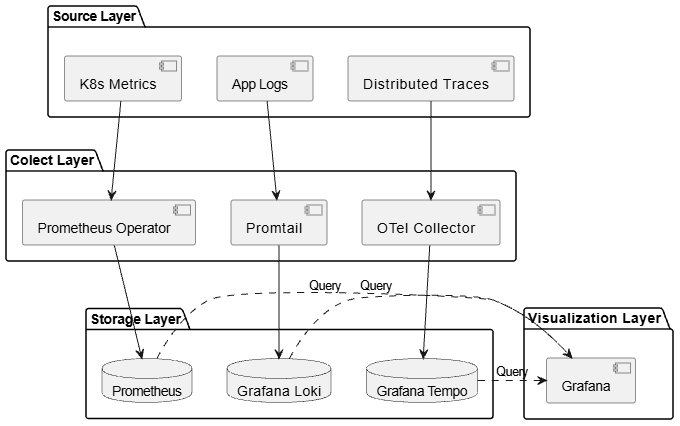
\includegraphics[width=1\linewidth]{images/cloud-computing/panoptes-layers.png}
    \par\medskip\ABNTEXfontereduzida\selectfont\textbf{Source:} The Author \par\medskip
    \label{fig:panoptes-data-layers}
\end{figure}

For numerical time-series data, Prometheus is the \textit{de facto} standard in the Cloud Native Computing Foundation (CNCF) ecosystem \cite{yeruva_2021}. The reference architecture uses the pull model, where the Prometheus server performs the scraping of metrics exposed by the `/metrics` endpoints of the services and Kubernetes itself (via kube-state-metrics) \cite{dubey_2021}.

For horizontal pod scalability (HPA - Horizontal Pod Autoscaler), the Metrics Server is an essential component that aggregates resource usage metrics and makes them available via the Kubernetes metrics API \cite{muschko_2020}.

In distributed environments, logs cannot be accessed in isolation via `kubectl logs' in production. The architecture requires a log forwarder (such as Fluentd or Fluent Bit) to centralize output streams. These logs must be processed to extract structured fields correlated with Kubernetes metadata before being sent to a storage backend (such as Elasticsearch, Loki, or OpenSearch) \cite{wilkins_2019,ibryam_2019}.

To understand latency and request flow between microservices, distributed tracing is mandatory. Tools like Jaeger or Tempo receive spans generated by applications instrumented via OpenTelemetry. The OpenTelemetry Collector component plays a crucial role here, receiving traces via protocols such as OTLP, processing them (e.g., sampling and filtering sensitive data), and exporting them to the visualization backend \cite{hausenblas_2023,young_2024}.

OpenTelemetry (OTel) acts as the unifying layer in the reference architecture. It solves the problem of tool fragmentation by providing a single standard for APIs, SDKs, and protocols (OTLP) \cite{flanders_2024}.

A central component is the OpenTelemetry Collector, which can be deployed in two main modes in Kubernetes: Agent Mode (DaemonSet) or Gateway Mode (Deployment). In the first case, it runs on each node to collect logs and metrics from the host, minimizing network latency. In the second one, it is a centralized cluster of collectors that receives data from the agents, performs heavy processing (such as tail-based sampling and aggregation), and exports to the back. OpenTelemetry has become so relevant that cloud vendors like Google have adopted the OTLP protocol to create their own telemetry API \cite{google_cloud_observability_2024}.

A fundamental requirement for the PANOPTES architecture is to ensure semantic integration between the observability pillars without excessively burdening cluster resources, directly addressing the secondary research questions of this thesis. Consequently, the selection of the storage and visualization backends was not arbitrary, but rather guided by strict scientific and engineering principles concerning resource efficiency, scalability, and data correlation.

\begin{itemize}
    \item \textbf{Prometheus (Pull-Based Model vs. Push Agents):} While solutions like InfluxDB offer robust time-series capabilities, Prometheus was selected due to its pull-based scraping architecture. Scientifically, in highly distributed cloud-native systems, a pull model prevents the monitoring backend from being overwhelmed (a monitoring-induced DDoS) during traffic spikes, as the central server dictates the ingestion rate \cite{beyer_2016}. Furthermore, relying on heavy push-agents within microservices consumes valuable CPU and memory on the application pods to buffer, batch, and transmit data, which frequently leads to application degradation under heavy monitoring loads \cite{usman_2022, weng_2018}. Prometheus integrates natively with the Kubernetes API and \texttt{kube-state-metrics}, pulling state data directly from HTTP endpoints with minimal application-level overhead.
    
    \item \textbf{Loki (Label Indexing vs. Full-Text Indexing):} Traditional log aggregation architectures rely heavily on the ELK stack (Elasticsearch, Logstash, Kibana). However, Elasticsearch employs full-text indexing (inverted indices) for every log line, which often requires a storage footprint and memory allocation (JVM heap) larger than the raw data itself, severely impacting system scalability \cite{he_2021}. Loki mitigates this by indexing only the metadata (labels) and compressing the raw logs into sequential chunks. This architectural choice drastically reduces storage I/O and memory overhead, a critical factor for resource-constrained environments \cite{araujo_2024}. Moreover, it guarantees that logs share the exact same label taxonomy as Prometheus metrics, enabling seamless correlation without the computational cost of parsing every token.
    
    \item \textbf{Tempo (Object Storage vs. Heavy Databases):} While Jaeger is a historically significant distributed tracing tool, it typically relies on resource-intensive backend databases like Cassandra or Elasticsearch to maintain complex secondary indices for span lookups. This introduces a massive write-amplification problem and high RAM requirements to handle the throughput of trace spans, a well-documented bottleneck in distributed tracing architectures at scale \cite{kaldor_2017, sambasivan_2016}. Grafana Tempo was selected because it eliminates this dependency by buffering traces in memory and writing them as columnar blocks directly to cost-effective Object Storage (e.g., MinIO or S3). By offloading the discovery phase to Loki and Prometheus (which provide the \texttt{traceID}), Tempo bypasses the need for a dedicated indexing database entirely, providing a highly scalable tracing backend with a significantly lower operational footprint.
\end{itemize}

Having established that observability in Kubernetes is not merely a collection of isolated signals, but a complex integration challenge, we must now justify the architectural decisions that constitute the PANOPTES framework. The theoretical landscape described above highlights a clear tension: while metrics, logs, and traces are conceptually distinct, their effective use for fault diagnosis requires a high degree of semantic correlation. 

However, as discussed, standard Kubernetes installations often fail to provide this correlation, leaving practitioners with fragmented data silos that hinder root cause analysis. To bridge the gap between these theoretical observability pillars and a practical, resource-efficient diagnostic tool, the following section explicitly maps the technical design choices of PANOPTES to the overarching research objectives. This alignment demonstrates that each selected component—from instrumentation standards to storage backends—is not incidental, but a deliberate decision aimed at answering the specific Research Questions posed in Chapter \ref{chap:intro}.